\documentclass{article}
\usepackage{graphicx}
\usepackage{minted}
\usepackage{array}
\renewcommand*{\arraystretch}{2}




\title{SMBUD 2021 - Project work 3}
\author{\\Aman Gabba - 10793117 \\
Andrea Cerasani - 10680486
\\Giovanni Demasi - 10656704
\\Pasquale Dazzeo - 10562130
\\Vlad Marian Cimpeanu - 10606922}
\date{ \begin{figure}[b] \centering 
\includegraphics[scale=0.2]{Logo Polimi.png} \end{figure}
 }
\usepackage[dvipsnames]{xcolor}

\usepackage{ifxetex}
\usepackage{ifluatex}
\newif\ifxetexorluatex % a new conditional starts as false
\ifnum 0\ifxetex 1\fi\ifluatex 1\fi>0
   \xetexorluatextrue
\fi

\ifxetexorluatex
  \usepackage{fontspec}
\else
  \usepackage[T1]{fontenc}
  \usepackage[utf8]{inputenc}
  \usepackage[lighttt]{lmodern}
\fi

\usepackage{textcomp}
\usepackage{xcolor}
\usepackage{listings}
\usepackage{upquote}

\definecolor{keyword}{HTML}{2771a3}
\definecolor{pattern}{HTML}{b53c2f}
\definecolor{string}{HTML}{be681c}
\definecolor{relation}{HTML}{7e4894}
\definecolor{variable}{HTML}{107762}
\definecolor{comment}{HTML}{8d9094}

\lstset{
	numbers=none,
	stepnumber=1,
	numbersep=5pt,
	basicstyle=\small\ttfamily,
	keywordstyle=\color{keyword}\bfseries\ttfamily,
	commentstyle=\color{comment}\ttfamily,
	stringstyle=\color{string}\ttfamily,
	identifierstyle=,
	showstringspaces=false,
	aboveskip=3pt,
	belowskip=3pt,
	columns=flexible,
	keepspaces=true,
	breaklines=true,
	captionpos=b,
	tabsize=2,
	frame=none,
}

\lstset{upquote=true}

\lstdefinelanguage{cypher}
{
	morekeywords={
		GET, POST
	}
}


\newcommand{\mycdots}{\cdot\!\cdot\!\cdot}
\lstset{language=cypher,
	literate=*
	{...}{$\mycdots$}{1}
	{theta}{$\theta$}{1}
}
\lstset{escapeinside={<@}{@>}}


\begin{document}

\maketitle
\thispagestyle{empty}

\newpage

\tableofcontents

\newpage

\section{Introduction}

\subsection{Problem Specification}
The aim of this project was to design, store and query data on a NoSQL DB supporting a data analysis scenario over data about COVID-19 vaccination statistics. The purpose is that of building a comprehensive database of vaccinations.

A vaccinations dataset has been suggested, with the purpose to pick a time interval of at least 3 months from it and, by using an ElasticSearch installation, import the data, apply the appropriate schema design choices, implement some queries aiming at exploring the data statistics and design a basic visualization dashboard of the results.

\subsection{Hypothesis}
The assumptions taken into account are the following:

\begin{itemize}


\item It is assumed that people who completed the vaccination cycle belong to the following categories:
\begin{itemize}
    \item have taken two vaccine doses
    \item have taken a Janssen dose
    \item have taken a vaccine dose after previous infection
\end{itemize}
\item A person is considered vaccinated if he has already taken at least one dose or has already taken a vaccine dose after previous infection.
\item A person who has been previously infected is not supposed to take any second vaccination dose.
\end{itemize}
%\newpage
%\section{ER diagram}
%The designed ER diagram contains the following entities: Person, Place, Authorized body, Certificate, Event and Sanitary operator. Nurse and Doctor have been designed as sub-entities of Sanitary Operator, Vaccine and Swab have been designed as sub-entities of Certificate and the Recovery entity is related to a swab.

%Every person, identified by an unique tax code, can face some events, like for instance a vaccination, in determinates places with unique GPS coordinates. Through an event a person can obtain a certificate with unique UCI useful for checking its valitidy. Every certification is issued by an authorized issuer and all the events are performed by prepared sanitary operators.

\hfill\break
\newpage

%\hfill\break
%\begin{center}
%\includegraphics[scale=0.155]{document_diagram.png}
%\end{center}
\newpage
\section{Datasets}
Two different datasets has been used for analysis purposes. A description of both can be found below.
\subsection{Vaccine administration dataset}
The Dataset used for the project is named {\fontfamily{qcr}\selectfont"somministrazioni-vaccini-latest.csv"} and it has been downloaded from the {\fontfamily{qcr}\selectfont"dati"} folder from the official Italian Government Github repository at the following link :\\ \url{https://github.com/italia/covid19-opendata-vaccini}.
\subsubsection{Schema}
\label{subsec:vaccination schema}
This dataset contains information about administered vaccines in Italy and it is made by the following fields:
\hfill\break
\begin{center}
\begin{tabular}{ |m{4cm}|m{2cm}|m{4.5cm}|}
  \hline
  \bfseries{Field} & \bfseries{Data type} & \bfseries{Description} \\
  \hline\hline
  area & string & Code of the delivery region\\
    \hline
      supplier & string & Complete name of the supplier of the vaccine\\
    \hline
          administration date & datetime & Administration date of the vaccines\\
              \hline
          age group & string & Age group to which the subjects to whom the vaccine were administered belong\\
                        \hline
          male count & integer & Number of vaccinations administered to males per day, region and age group\\
                        \hline
          female count & integer & Number of vaccinations administered to females per day, region and age group\\
    \hline
  first doses & integer & Number of people administered with the first dose\\
    \hline
  second doses & integer & Number of people administered with the second dose\\
    \hline

\end{tabular}
\end{center}

\newpage
\begin{center}
\begin{tabular}{ |m{4cm}|m{2cm}|m{4.5cm}|}
\hline
  post infection doses & integer & Number of administrations given to subjects with previous covid-19 infection in the 3-6 month period and who, therefore, conclude the vaccination cycle with a single dose\\
    \hline
  booster doses & integer & Number of people administered with an additional dose/recall\\
    \hline
  NUTS1 code & string & European classification of NUTS territorial units: NUTS level 1\\
    \hline
  NUTS2 code & string & European classification of NUTS territorial units: NUTS level 2\\
    \hline
  ISTAT region code & integer & ISTAT code of the Region\\
    \hline
  region name & string & Standard denomination of the area (where necessary bilingual denomination)\\
  \hline
  \end{tabular}
\end{center}
\hfill\break
\hfill\break


%The dataset period taken into consideration for statistical purposes is the one that goes from the first day of the year 2021 to the last day of September 2021.

\newpage
\subsection{Istat population dataset}
As optional point of this project, analysis has been integrated with another dataset which contains information about the Italian population, like number of people per age range and region or number of people per gender per region. The dataset has been downloaded from a Covid-19 related Github repository at the following link: \url{https://github.com/pcm-dpc/COVID-19}, it is located in the {\fontfamily{qcr}\selectfont"dati-statistici-riferimento"} folder and it is the one named {\fontfamily{qcr}\selectfont"popolazione-istat-regione-range.csv"}.

\subsubsection{Schema}
This dataset contains information about population number per region and age range in Italy. It is made by the following fields:
\hfill\break
\begin{center}
\begin{tabular}{ |m{4cm}|m{2cm}|m{4.5cm}|}
  \hline
  \bfseries{Field} & \bfseries{Data type} & \bfseries{Description} \\
  \hline\hline
  ISTAT region code & integer & ISTAT code of the Region\\
  \hline
  NUTS1 code & string & European classification of NUTS territorial units: NUTS level 1\\
    \hline
      NUTS1 description & string & Cardinal direction based on the NUTS1 code\\
    \hline
          NUTS2 code & string & European classification of NUTS territorial units: NUTS level 2\\
              \hline
                        region name & string & Standard denomination of the area (where necessary bilingual denomination)\\
                        \hline
          area & string & Code of the region\\
                        \hline
          region latitude & float & Latitude coordinate of the region\\
                        \hline
          region longitude & float & Longitude coordinate of the region\\
    \hline

\end{tabular}
\end{center}

\newpage
\begin{center}
\begin{tabular}{ |m{4cm}|m{2cm}|m{4.5cm}|}
\hline
  age range & string & Age range to which the population numbers refers\\
    \hline
  male count & integer & Number of males in the population, per region and age range\\
    \hline

  female count & integer & Number of females in the population, per region and age range\\
    \hline
  total count & integer & Number of males plus females in the population, per region and age range\\
    \hline
  \end{tabular}
\end{center}
\hfill\break

\subsection{Other considerations}
The data types written in the schema tables are the 'original' ones, so the ones used by the datasets creators.

The same data types have been used to implement and use the dataset in ElasticSearch because they well represent the different parameters, so no changes were needed, except for the ISTAT region code field.
It is better to keep all the ISTAT region codes as keywords instead of numbers for the following reason:

they are numbers but for compatibility reasons they should be considered as keywords. In Kibana, there is the possibility to associate data to regions according to ISTAT code convention, by the way, the format used by Kibana is the following "01, 02, 03, 04, ...", thus, if ISTAT codes are imported as numbers they will not be compatible with that convention as Kibana will find the following codes "1, 2, 3, 4, ...".

As the original datasets does not follow the Kibana convention, it has been adapted through the script {\fontfamily{qcr}\selectfont"dataset\_cleaner.py"}.

\hfill\break
Both datasets used have Istat region code as field, to understand what it is it is suggested to visit the following link: \\ \url{https://en.wikipedia.org/wiki/NUTS\_statistical\_regions\_of\_Italy}.
\hfill\break
\hfill\break
When the two datasets will be imported, both created indexes will use Istat region code to identify a region. The original dateset used for istat\_population did not assign a code to Trentino region (04), instead it assigned codes for Bolzano(21) and Trento (22) provinces. For this reason codes have been corrected in order to link the two indexes.


\newpage
\section{Queries and Commands}
In the following chapter all the queries and commands parameters (part of the code to substitute with desired values) will be highlighted with {\color{magenta}{magenta}} bold text.

Some parameters information can be useful for different queries or commands so they are written here to avoid writing them multiple times:
\begin{itemize}
    \item {\color{magenta}{Start date}} and {\color{magenta}{End date}} are, respectevely, the starting date of a period and the ending date of a period. Dates must be in the following format YYYY-MM-DD and, obviously, End date must be subsequent to Start date.
    \item {\color{magenta}{Date}} is a generic date and it must be in the following format YYYY-MM-DD.
    \item {\color{magenta}{Supplier}}, for coherence w.r.t other documents, must be one of the following: Moderna, Janssen, Pfizer/BioNTech or Vaxzevria (AstraZeneca).
    \item {\color{magenta}{Age range}} must follow one of this format: 12-19, x0-x9 or 90+ (where x is a number between 2 and 8)
\end{itemize}
\subsection{Queries}
The first eight queries refer only on the vaccination dataset. Instead, the last two queries refer to both vaccination and Istat population dataset.
\subsubsection{Delta vaccination per area}
For each region, this query returns the percentage of the difference between vaccinations of a given date and its precedent day, calculated with respect to the amount of vaccinations performed the day before.
If the vaccinations have increased, the percentage will be positive, negative otherwise.

This query has thought to be used during the current day, thus the parameters "{\color{magenta}{Date 1}}" and "{\color{magenta}{Date 2}}" should be respectively "now" and "now-1d/d". By the way, as the database is not up to date, the query will not be correctly performed, for this reason it is suggested to use the last dates available in the dataset which are "2021-12-22" and "2021-12-21".

\begin{lstlisting}[language=cypher, label=lst:cypher-example]

GET istat_vaccinations/_search
{
  "size" : 0,
  "aggs": {
    "group_by_area": {
      "terms": {
        "field": "nome_area"
      },
      "aggs": {
        "today_vaccinations" :{
          "filter": {
            "term" : {
              "data_somministrazione": "<@\textbf{\color{magenta}{Date 1}}@>"
            }
          },
          "aggs": {
            "amount": {
              "sum": {
                "script": {
                  "source": "doc['sesso_maschile'].value + doc['sesso_femminile'].value"
                }
              }
            }
          }
        },
        "yesterday_vaccinations" : {
          "filter": {
            "term" : {
              "data_somministrazione": "<@\textbf{\color{magenta}{Date 2}}@>"
            }
          },
          "aggs" : {
            "amount": {
              "sum" :{
                "script": {
                  "source": "doc['sesso_femminile'].value + doc['sesso_maschile'].value"
                }
              }
            }
          }
        },
        "delta_percentage" : {
          "bucket_script": {
            "buckets_path": {
              "today" : "today_vaccinations>amount",
              "yesterday" : "yesterday_vaccinations>amount"
            },
            "script": "(params.today - params.yesterday) / params.yesterday * 100"
          }
        }
      }
    }
  }
}

\end{lstlisting}
\newpage
\subsubsection{Percentage full covered vaccinations}
The following query calculates the percentage of people which has already completed the vaccination cycle, starting from the date the vaccinations started. The percentage is calculated with respect to all the vaccinated people, so everyone that has already received at least one dose.
The cycle is considered completed if a person:
\begin{itemize}
\item is vaccinated with Janssen vaccine.
\item has already received the second dose.
\end{itemize}

\begin{lstlisting}[language=cypher, label=lst:cypher-example]

GET istat_vaccinations/_search
{
  "size" : 0,
  "aggs":{
    "group_by": {
      "date_range": {
        "field": "data_somministrazione",
        "ranges": [
          {
            "from": "2020-12-27",
            "to": "now"
          }
        ]
      },
      "aggs": {
        "sum_first_dose": {
          "sum" :{
            "field" : "prima_dose"
          }
        },
        "sum_second_dose" : {
          "sum" : {
            "field" : "seconda_dose"
          }
        },
        "sum_Janssen": {
          "filter": {
            "term" : {
              "fornitore": "Janssen"
            }
          },
          "aggs": {
            "amount" : {
              "sum" : {
                "field": "prima_dose"
              }
            }
          }
        },
        "after_infection": {
          "sum": {
            "field" : "pregressa_infezione"
          }
        },
        "full_coverage_percentage" : {
          "bucket_script": {
            "buckets_path": {
              "first_dose": "sum_first_dose",
              "second_dose": "sum_second_dose",
              "janssen_vax": "sum_Janssen>amount",
              "infection": "after_infection"
            },
            "script": "(params.second_dose + params.janssen_vax + params.infection)/ (params.first_dose + params.infection) * 100"
          }
        }
      }
    }
  }
}

\end{lstlisting}
\subsubsection{Vaccination trend}
For each day, this query returns the vaccinations performed.

\begin{lstlisting}[language=cypher, label=lst:cypher-example]

GET istat_vaccinations/_search
{
  "size" : 0,
  "aggs": {
    "group_by_date": {
      "date_histogram": {
        "field": "data_somministrazione",
        "interval": "day"
      },
      "aggs": {
        "sum_vaccinations": {
          "sum": {
            "script": {
              "source": "doc['sesso_maschile'].value + doc['sesso_femminile'].value"
            }
          }
        }
      }
    }
  }
}

\end{lstlisting}
\newpage
\subsubsection{Brand administrated vaccines percentage for a given period}
The following query, given a period of time, returns the percentage of the administrated vaccines per brand.

\begin{lstlisting}[language=cypher, label=lst:cypher-example]

GET istat_vaccinations/_search
{
  "size":0,
  "aggs": {
    "group_by_date": {
      "date_range": {
        "field": "data_somministrazione",
        "ranges": [
          {
            "from": "<@\textbf{\color{magenta}{Start date}}@>",
            "to": "<@\textbf{\color{magenta}{End date}}@>"
          }
        ]
      },
      "aggs": {
        "total_vaccinations": {
          "sum": {
            "script": {
              "source": "doc['sesso_maschile'].value + doc['sesso_femminile'].value"
            }
          }
        },
        "group_by_brand": {
          "terms": {
            "field": "fornitore"
          },
          "aggs": {
            "amount": {
              "sum": {
                "script": {
                  "source": "doc['sesso_maschile'].value + doc['sesso_femminile'].value"
                }
              }
            }
          }
        },
        "astrazeneca_percentage": {
          "bucket_script": {
            "buckets_path": {
              "tot": "total_vaccinations",
              "astra": "group_by_brand['Vaxzevria (AstraZeneca)']>amount"
            },
            "script": "(params.astra / params.tot) * 100"
          }
        },
        "moderna_percentage": {
          "bucket_script": {
            "buckets_path": {
              "tot": "total_vaccinations",
              "moderna": "group_by_brand['Moderna']>amount"
            },
            "script": "(params.moderna / params.tot) * 100"
          }
        },
        "pfizer_percentage":{
          "bucket_script": {
            "buckets_path": {
              "tot": "total_vaccinations",
              "pfizer": "group_by_brand['Pfizer/BioNTech']>amount"
            },
            "script": "(params.pfizer / params.tot) * 100"
          }
        },
        "janssen_percentage": {
          "bucket_script": {
            "buckets_path": {
              "tot": "total_vaccinations",
              "janssen": "group_by_brand['Janssen']>amount"
            },
            "script": "(params.janssen / params.tot) * 100"
          }
        }
      }
    }
  }
}

\end{lstlisting}
\newpage
\subsubsection{Percentages of administrated doses,  by dose number, for a given period}
This query returns the percentage of first doses, second doses and boosters administrated during the given period.

\begin{lstlisting}[language=cypher, label=lst:cypher-example]

GET istat_vaccinations/_search
{
  "size" : 0,
  "aggs": {
    "group_by_date": {
      "date_range": {
        "field": "data_somministrazione",
        "ranges": [
          {
            "from": ""<@\textbf{\color{magenta}{Start date}}@>"",
            "to": ""<@\textbf{\color{magenta}{End date}}@>""
          }
        ]
      },
      "aggs": {
        "first_doses": {
          "sum": {
            "script": {
              "source": "doc['prima_dose'].value + doc['pregressa_infezione'].value"
            }
          }
        },
        "second_doses": {
          "sum": {
            "field" : "seconda_dose"
          }
        },
        "boosters": {
          "sum": {
            "field" : "dose_addizionale_booster"
          }
        },
        "First_dose_Percentage" : {
          "bucket_script": {
            "buckets_path": {
              "First": "first_doses",
              "Second": "second_doses",
              "Booster": "boosters"
            },
            "script": "(params.First)/ (params.First + params.Second + params.Booster) * 100"
          }
        },
        "Second_dose_Percentage" : {
          "bucket_script": {
            "buckets_path": {
              "First": "first_doses",
              "Second": "second_doses",
              "Booster": "boosters"
            },
            "script": "(params.Second)/ (params.First + params.Second + params.Booster) * 100"
          }
        },
        "Booster_Percentage" : {
          "bucket_script": {
            "buckets_path": {
              "First": "first_doses",
              "Second": "second_doses",
              "Booster": "boosters"
            },
            "script": "(params.Booster)/ (params.First + params.Second + params.Booster) * 100"
          }
        }
      }
    }
  }
}

\end{lstlisting}
\newpage
\subsubsection{Vaccination percentage per age range for a given period}
The following query returns the percentage of vaccinated people per age range during the given period.

\begin{lstlisting}[language=cypher, label=lst:cypher-example]

GET istat_vaccinations/_search
{
  "size" : 0,
  "aggs": {
    "group_by_date": {
      "date_range": {
        "field": "data_somministrazione",
        "ranges": [
          {
            "from": "<@\textbf{\color{magenta}{Start date}}@>",
            "to": "<@\textbf{\color{magenta}{End date}}@>"
          }
        ]
      },
      "aggs": {
        "age_range": {
          "terms": {
            "field": "fascia_anagrafica"
          },
          "aggs": {
            "amount":{
              "sum": {
                "script": {
                  "source": "doc['sesso_maschile'].value + doc['sesso_femminile'].value"
                }
              }
            }
          }
        },
        "total": {
          "sum": {
            "script": {
              "source": "doc['sesso_maschile'].value + doc['sesso_femminile'].value"
            }
          }
        },
        "teen_percentage" : {
          "bucket_script": {
            "buckets_path": {
              "Teen": "age_range['12-19']>amount",
              "tot": "total"
            },
            "script": "(params.Teen) / (params.tot) * 100"
          }
        },
        "20s_percentage" : {
          "bucket_script": {
            "buckets_path": {
              "20": "age_range['20-29']>amount",
              "tot":"total"
            },
            "script": "(params.20)/ (params.tot) * 100"
          }
        },
        "30s_percentage" : {
          "bucket_script": {
            "buckets_path": {
              "30": "age_range['30-39']>amount",
              "tot": "total"
            },
            "script": "(params.30)/ (params.tot) * 100"
          }
        },
        "40s_percentage" : {
          "bucket_script": {
            "buckets_path": {
              "40": "age_range['40-49']>amount",
              "tot": "total"
            },
            "script": "(params.40)/ (params.tot) * 100"
          }
        },
        "50s_percentage" : {
          "bucket_script": {
            "buckets_path": {
              "50": "age_range['50-59']>amount",
              "tot": "total"
            },
            "script": "(params.50)/ (params.tot) * 100"
          }
        },
        "60s_percentage" : {
          "bucket_script": {
            "buckets_path": {
              "60": "age_range['60-69']>amount",
              "tot": "total"
            },
            "script": "(params.60)/ (params.tot) * 100"
          }
        },
        "70s_percentage" : {
          "bucket_script": {
            "buckets_path": {
              "70": "age_range['70-79']>amount",
              "tot": "total"
            },
            "script": "(params.70)/ (params.tot) * 100"
          }
        },
        "80s_percentage" : {
          "bucket_script": {
            "buckets_path": {
              "80": "age_range['80-89']>amount",
              "tot": "total"
            },
            "script": "(params.80)/ (params.tot) * 100"
          }
        },
        "90+_percentage" : {
          "bucket_script": {
            "buckets_path": {
              "90": "age_range['90+']>amount",
              "tot": "total"
            },
            "script": "(params.90)/ (params.tot) * 100"
     	    }
        }
      }
    }
  }
}

\end{lstlisting}
\newpage
\subsubsection{Regions ranking per number of vaccinations for a given day}
The following query returns the ranking of regions per number of vaccines administrated, for a given date.

\begin{lstlisting}[language=cypher, label=lst:cypher-example]

GET istat_vaccinations/_search
{
  "size" : 0,
  "query": {
    "bool": {
      "must":{
        "term": {
          "data_somministrazione": {
            "value": "<@\textbf{\color{magenta}{Date}}@>"
          }
        }
      }
    }
  },
  "aggs": {
    "group_by_region": {
      "terms": {
        "field": "nome_area"
        , "size": 21
      },
      "aggs": {
        "sum_vaccinations": {
          "sum": {
            "script": {
              "source": "doc['sesso_maschile'].value + doc['sesso_femminile'].value"
            }
          }
        },
        "sort_by_vaccinations":{
          "bucket_sort": {
            "sort": [{ "sum_vaccinations": { "order": "desc" } }]
          }
        }
      }
    }
  }
}

\end{lstlisting}
\newpage
\subsubsection{Percentage of booster administrated}
The following query returns percentage of people who received booster dose over those who completed the vaccination cycle at least 5 months ago and are potentially subject to booster dose. The considered candidate people are the ones who belongs to the following categories:
\begin{itemize}
    \item Completed the vaccinations cycle with two vaccines doses
    \item Vaccinated with Janssen
    \item Recoveded and subsequently vaccined
\end{itemize}

\begin{lstlisting}[language=cypher, label=lst:cypher-example]

GET istat_vaccinations/_search
{
  "size" : 0,
  "aggs": {
    "all_matching_docs": {
      "filters": {
        "filters": {
          "all": {
            "match_all": {}
          }
        }
      },
      "aggs":{
        "sum_booster":{
          "sum": {
            "field": "dose_addizionale_booster"
          }
        },
        "booster_candidates": {
          "filter": {
            "range": {
              "data_somministrazione": {
                "lte": "2021-12-22||-5M"
              }
            }
          },
          "aggs": {
            "sum_second_dose" : {
              "sum" : {
                "field" : "seconda_dose"
              }
            },
            "sum_janssen": {
              "filter": {
                "term" : {
                  "fornitore": "Janssen"
                }
              },
              "aggs": {
                "amount" : {
                  "sum" : {
                    "field": "prima_dose"
                  }
                }
              }
            },
            "sum_previous_infection": {
              "sum" : {
                "field" : "pregressa_infezione"
              }
            }
          }
        },
        "booster_percentage" : {
          "bucket_script": {
            "buckets_path": {
              "second_dose" : "booster_candidates>sum_second_dose",
              "janssen" : "booster_candidates>sum_janssen>amount",
              "previous_infection" : "booster_candidates>sum_previous_infection",
              "booster" : "sum_booster"
            },
            "script": "params.booster / (params.second_dose + params.janssen + params.previous_infection) * 100"
          }
        }
      }
    }
  }
}

\end{lstlisting}
\newpage
\subsubsection{Percentage of vaccinated people per region}
This query uses both datasets and returns the percentage of vaccinated people per region over its total population.

\begin{lstlisting}[language=cypher, label=lst:cypher-example]

GET /istat*/_search
{
  "size" : 0,
  "aggs":{
    "group_by_region":{
      "terms" : {
        "field" : "codice_regione_ISTAT"
      },
      "aggs": {
        "total_first_doses": {
          "sum": {
            "field" : "prima_dose"
          }
        },
        "total_previous_infections":{
          "sum":{
            "field": "pregressa_infezione"
          }
        },
        "total_people": {
          "sum": {
            "field" : "totale_generale"
          }
        },
        "ratio_vaccinated_people": {
          "bucket_script": {
            "buckets_path": {
	            "first": "total_first_doses",
              "total" : "total_people",
              "inf": "total_previous_infections"
            },
            "script":"((params.first + params.inf)/params.total)*100"
         }
        }
      }
    }
  }
}

\end{lstlisting}
\newpage
\subsubsection{Query 10}
The following query...

\begin{lstlisting}[language=cypher, label=lst:cypher-example]

CODE

\end{lstlisting}
\newpage
\subsection{Commands}
All the fields of the following commands are parameters, some will be highlighted in magenta, other won't, due to their exhaustive explanation that can be found in section \ref{subsec:vaccination schema}.
\subsubsection{Create new document}
This command creates a new database document. Here it is reported a complete example.

\begin{lstlisting}[language=cypher, label=lst:cypher-example]

POST /istat_vaccinations/_doc
{
  "data_somministrazione": "<@\textbf{\color{magenta}{Date}}@>",
  "fornitore": "<@\textbf{\color{magenta}{Supplier}}@>",
  "area": "ABR",
  "fascia_anagrafica": "<@\textbf{\color{magenta}{Age range}}@>",
  "sesso_maschile": "1",
  "sesso_femminile": "1",
  "prima_dose": "1",
  "seconda_dose": "2",
  "pregressa_infezione": "0",
  "dose_addizionale_booster": "0",
  "codice_NUTS1": "ITF",
  "codice_NUTS2": "ITF1",
  "codice_regione_ISTAT": "13",
  "nome_area": "Abruzzo"
}

\end{lstlisting}
\newpage
\subsubsection{Update of number of first doses}
This command, given a specific document id, update the number of first doses. Here it is reported both the command and also the query useful to find a document it.
\hfill\break
\hfill\break
\textbf{Find document id}
\hfill\break
With this query it is possible to find a document id by specifing these fields: data\_somministrazione, codice\_regione\_ISTAT, fornitore and fascia\_anagrafica.

\begin{lstlisting}[language=cypher, label=lst:cypher-example]

GET /istat_vaccinations/_search
{
  "query": {
    "bool": {
      "must": [
        {
          "match": {
            "data_somministrazione": "<@\textbf{\color{magenta}{Date}}@>"
          }
        },
        {
          "match": {
            "codice_regione_ISTAT": "13"
          }
        },
        {
          "match": {
            "fornitore": "<@\textbf{\color{magenta}{Supplier}}@>"
          }
        },
        {
          "match": {
            "fascia_anagrafica": "<@\textbf{\color{magenta}{Age Range}}@>"
          }
        }
      ]
    }
  }
}
\end{lstlisting}
\hfill\break
\textbf{First doses update}
\hfill\break
Now it is possible to update the number of doses of the document found.

\begin{lstlisting}[language=cypher, label=lst:cypher-example]

POST /istat_vaccinations/_update/8FjS_H0BhG8f5U0W2n46
{
  "doc": {
    "prima_dose" : 3000
} }

\end{lstlisting}
\newpage

\section{Dashboard description}
The Kibana Dashboard is made by different section, each focusing on a specific analysis.
Here there is a brief description of each part is given.

\subsection{Percentage of Vaccines brand per age range}
In this section a pie chart has been used to show two different things: in the inner layer there is the percentage of people vaccinated per age range, in the outer layer there is the percentage of brand vaccines used per age range.

\begin{center}
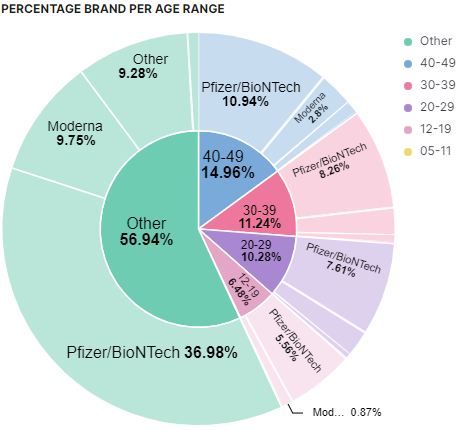
\includegraphics[scale=0.5]{perc_brand_age_range.png}
\end{center}

\subsection{First doses with proportion among vaccines brands}
This histogram, fixed a specific interval of time, returns the amount of first doses administrated for each week. In addition the histogram shows the division per vaccine brand for each week.

\begin{center}
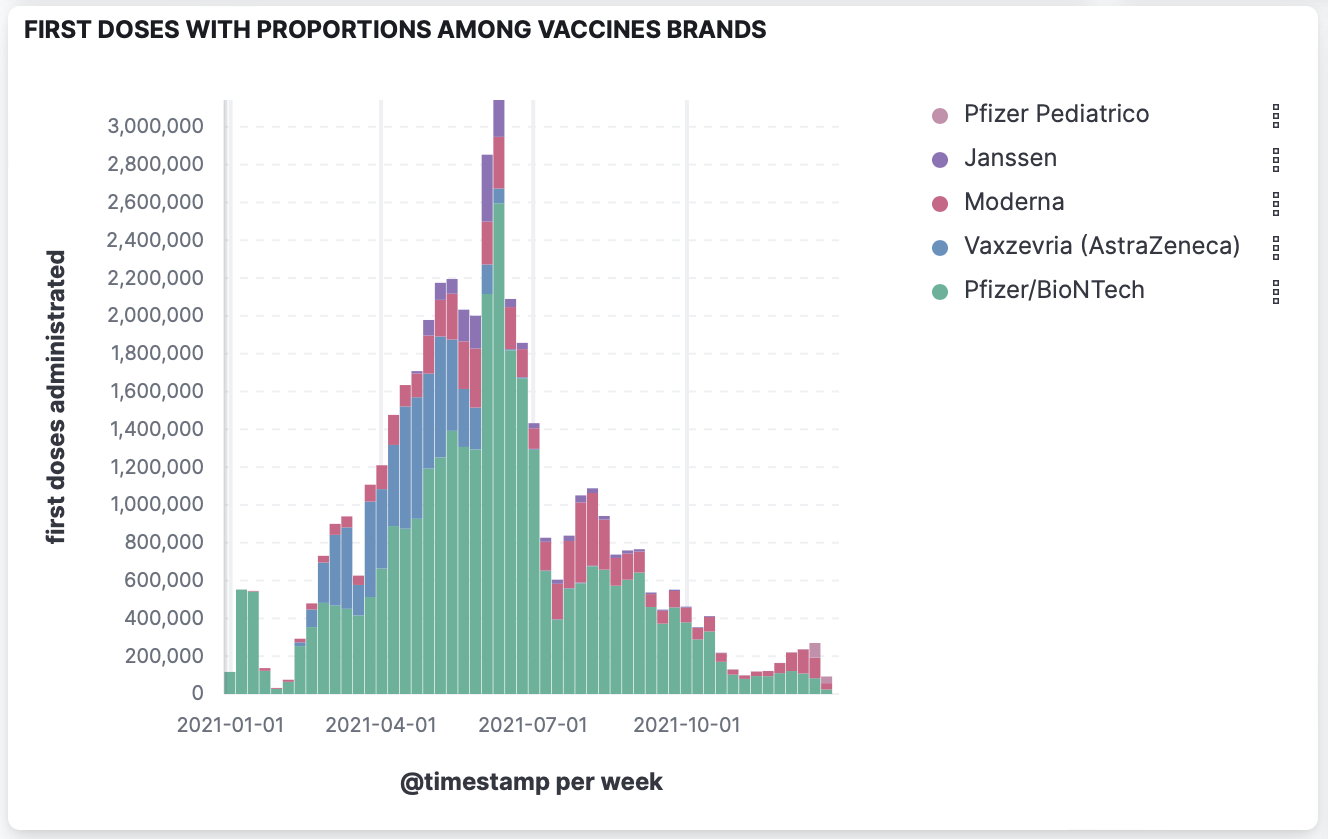
\includegraphics[scale=0.6]{first_doses_vacc_brand.png}
\end{center}

\subsection{Vaccinated people}
This section, given a specific period of time, returns the amount of people who have:
\begin{itemize}
    \item vaccinated at least once
    \item completed the vaccination cycle
    \item received the booster dose
\end{itemize}

\begin{center}
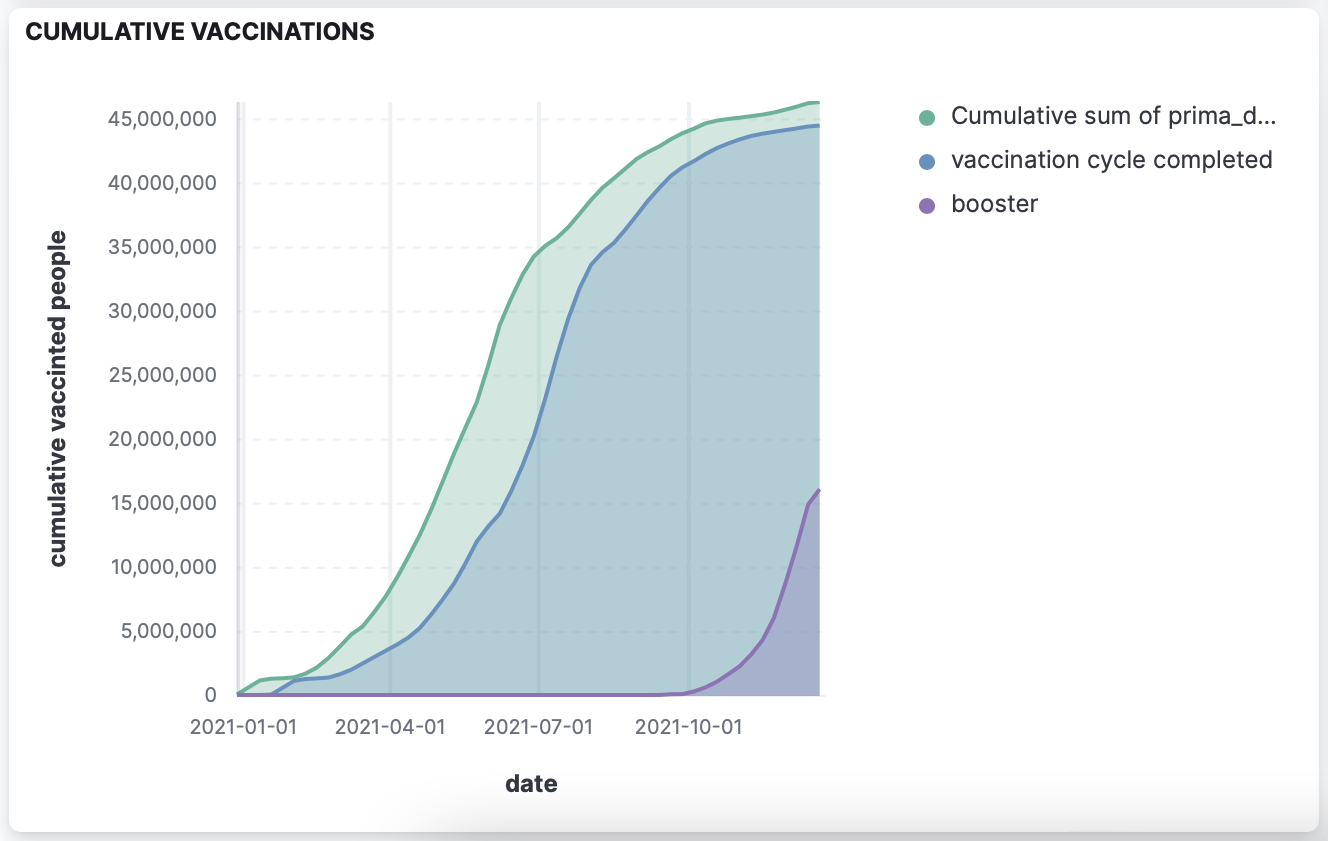
\includegraphics[scale=0.6]{cumulat_vacc.png}
\end{center}

\subsection{Vaccines administrated per region}
Here an histogram has been used to show the amount of people who vaccinated at least once for a specific range of time per region.

\begin{center}
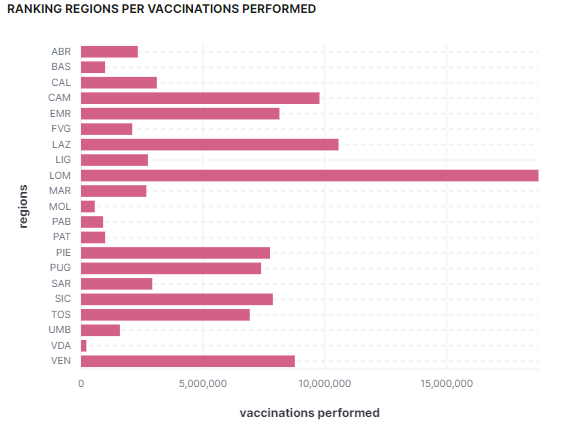
\includegraphics[scale=0.6]{ranking_regions.png}
\end{center}

\subsection{Vaccination administrated per day}
This diagram shows the amount of vaccinations administrated per day during a given range of time.

\begin{center}
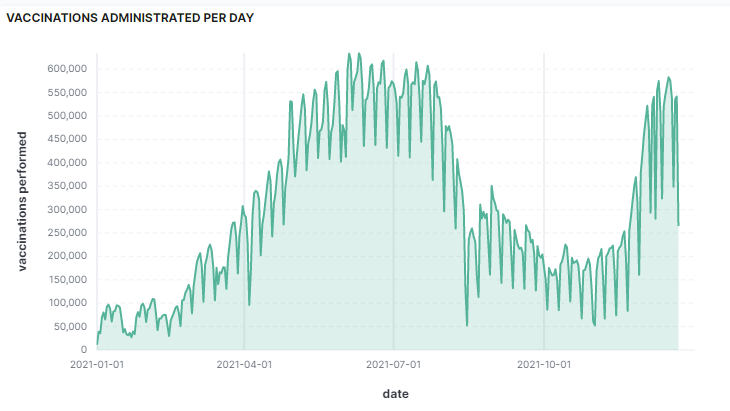
\includegraphics[scale=0.6]{vacc_adm_per_day.png}
\end{center}

\subsection{Who can take booster}
This histogram, returns the percentage of people who received the booster dose for each day. The percentage has been considered with respect to all the people who are eligible to receive the booster dose, so all the people who completed the vaccination cycle at least 5 months before the analyzed date.

\begin{center}
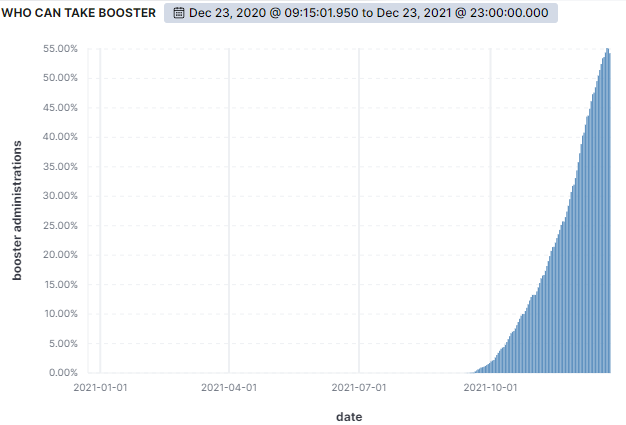
\includegraphics[scale=0.6]{who_booster.png}
\end{center}

\subsection{Delta percentage of vaccinations with respect to yesterday}
It returns the percentage of the difference between vaccinations of a given date and its precedent day, calculated with respect to the amount of vaccinations performed the day before.
If the vaccinations have increased, the percentage will be positive, negative otherwise.
This widget has meant to be used in real time, thus it should refers to the current date. By the way, as the database is not up to date, the widget shows the last date available in the dataset which is "2021-12-22".

\begin{center}
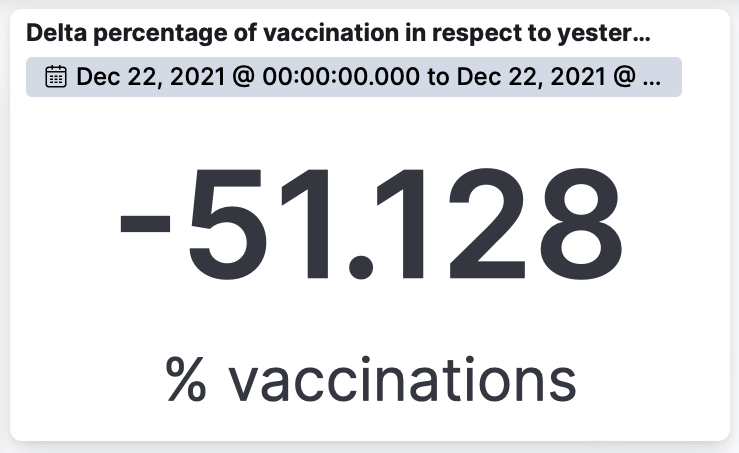
\includegraphics[scale=0.6]{delta_perc.png}
\end{center}

\subsection{Vaccinations type distribution during a given interval of time}
Given period of time, it represents the distribution among first doses, second doses and boosters for each week.

\begin{center}
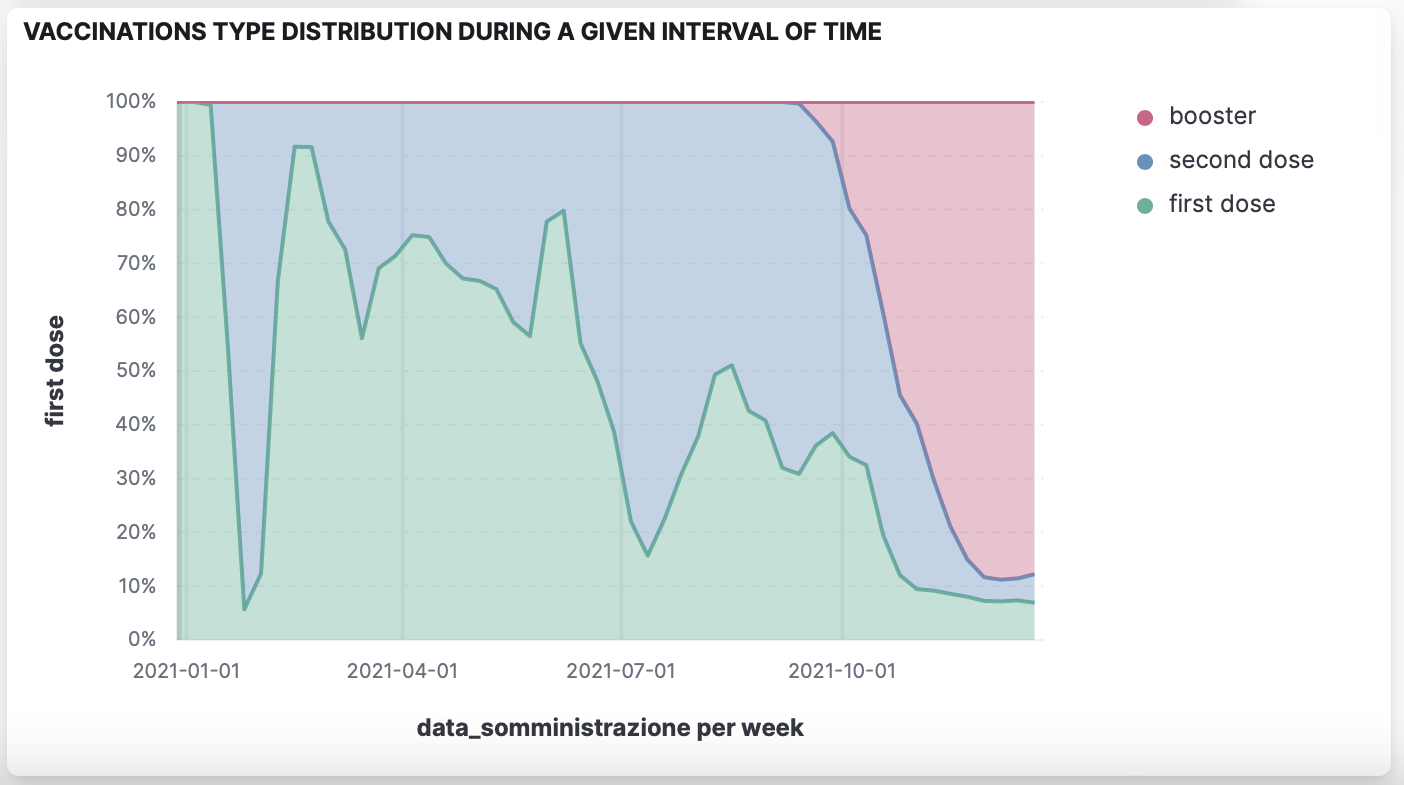
\includegraphics[scale=0.6]{vacc_distr.png}
\end{center}

\newpage

\section{User guide}

\subsection{Import data}
\subsubsection{Import vaccinations dataset}
After having opened Kibana, it is necessary to click on the {\fontfamily{qcr}\selectfont"upload file"} button present in the home page. Now the file named {\fontfamily{qcr}\selectfont"cleaned\_data.csv"} must be dragged and dropped in the opened page.

After that, the {\fontfamily{qcr}\selectfont"import"} button must be clicked. In the new page, in the advanced setting section, it is necessary to use the {\fontfamily{qcr}\selectfont"istat\_vaccinations"} index name. In the mapping section, {\fontfamily{qcr}\selectfont"codice\_regione\_ISTAT"} type must be replaced with "keyword"(line 16).

In the Ingest pipeline section, the conversion part of {\fontfamily{qcr}\selectfont"codice\_regione\_ISTAT"} (lines from number 36 to number 42, both included) must be deleted.
Then, by clicking the import button, vaccinations data will be successfully imported.

\subsubsection{Import Istat population dataset}
In order to import the Istat population dataset, it is necessary to repeat the same procedure described before. First, upload the {\fontfamily{qcr}\selectfont"new\_istat\_code.csv"} file and use {\fontfamily{qcr}\selectfont"istat\_population"} as index name. Then, apply the same changes in mapping section (line 13) and ingest pipeline section (lines from number 33 to number 39, both included) as shown before.


\subsection{Import dashboard}
After having opened Kibana it is necessary to go in the {\fontfamily{qcr}\selectfont"Stack management"} section. From this page, the {\fontfamily{qcr}\selectfont"Saved objects"} button present in the left bar, in the Kibana section, must be clicked. 

In the new page it is necessary to click the {\fontfamily{qcr}\selectfont"Import data"} button and then upload the {\fontfamily{qcr}\selectfont"dashboard.ndjson"} file. 

It may appear an index conflict, in this case it is important to select as index the one referred to {\fontfamily{qcr}\selectfont"istat\_vaccinations"}.
After that just click the {\fontfamily{qcr}\selectfont"Import"} button; the dashboard will now be visible in {\fontfamily{qcr}\selectfont"Dashboard"} section.

\newpage

\section{Conclusion}

Some interesting conclusions can be drawn from the development of this project:

Elasticsearch and Kibana are a perfect match to make different type of analysis about trends even by using a big amount of data.

Kibana makes Elasticsearch queries output really simple to understand and visualize, and it can be really helpful because in this way the analysis results can be understand even by those who doesn't have any knowledge about computer science.

\section{References and Sources}
\begin{itemize}
    %\item \url{Random-italian-person package: https://pypi.org/project/random-italian-person}
    %\item \url{PyMongo package: https://docs.mongodb.com/drivers/pymongo/}
    %\item \url{Flask package: https://flask.palletsprojects.com/en/2.0.x/}
    \item Elastic Guide: \url{https://www.elastic.co/guide/index.html}
    \item Italian Government repository: \url{https://github.com/italia/covid19-opendata-vaccini}
    
    %\item Overpass turbo API: https://wiki.openstreetmap.org/wiki/Overpass\_API
\end{itemize}



\end{document}